% Workshop submission: switchable-component ablation of a coding-agent harness.
%
% STYLE FILE: this compiles standalone with `article` so it can be checked
% without network access. For submission, uncomment the \usepackage line for
% the host workshop's current style file and delete the geometry/fonts block
% below. Workshop style files are reissued every year -- take the one linked
% from the workshop's own call, not a copy from elsewhere.
%
% \usepackage{neurips_20XX}      % or iclr_20XX_workshop, etc.

\documentclass[10pt]{article}

\usepackage[letterpaper,margin=1in]{geometry}
\usepackage{times}
\usepackage{amsmath,amssymb}
\usepackage{graphicx}
\usepackage{booktabs}
\usepackage{microtype}
\usepackage[numbers,sort&compress]{natbib}
\usepackage[hidelinks]{hyperref}
\usepackage{pgfplots}
\pgfplotsset{compat=1.18}
\usepackage{caption}
\captionsetup{font=small,labelfont=bf}

\title{Which Harness Components Actually Pay?\\
A Switchable-Component Ablation on Local Coding Agents}

% Anonymised for review. Replace for camera-ready.
\author{Anonymous Author(s)\\Anonymous Institution}
\date{}

\begin{document}
\maketitle

\begin{abstract}
The pass rate of a coding agent is a property of the model \emph{and} its harness --- the
code that builds context, exposes tools, caps output, and decides when work is done.
Published harnesses differ by more than twenty points on the same frontier model, but that
evidence is a leaderboard spread across independently engineered systems, not a controlled
ablation, and it says nothing about which \emph{component} pays. We build a harness whose
seven components are independently switchable, put the grader outside the agent's reach, and
run every configuration on locally served models. On a 720-episode grid (2 models $\times$ 9
configurations $\times$ 5 pinned seeds $\times$ 8 hidden-test tasks), the full bundle raises
Qwen~3.8~27B from 90.0\% to 95.0\%, a paired $\Delta$ of $+5.0$ points whose bootstrap 95\%
interval $[0.0, +10.0]$ includes zero. Three findings survive the intervals. First,
\textbf{the full bundle is not optimal for either model}: both peak at an ablation, not at
\texttt{full}. Second, the only interval in the entire one-flag ladder that excludes zero says
a component \emph{hurt} --- removing the output cap raises the weaker model by 10.0 points.
Third, the capability-by-harness interaction that motivates harness engineering is
\textbf{undetectable at this sample size}: all eight intervals include zero and disagree in
sign. We also report two ways this measurement can silently go wrong, both of which we hit: a
mid-grid protocol change inflated the same contrast to $+22.5$ points, and an API arm we tried
to add was censored by the endpoint in a way that correlated with task difficulty. The
artifact is 3{,}500 lines of dependency-free Python; every number here regenerates from one
command.
\end{abstract}

\section{Introduction}

A coding agent is a language model plus a loop. That loop decides what the model sees on turn
one, which tools it may call, how much of a tool result comes back, whether a repeated call is
blocked, and whether \texttt{finish} ends the episode or is returned with failing tests. It is
the harness, and changing it while holding the model fixed moves pass rate by tens of points
\citep{metaharness,terminalbench}. Practitioners add a system prompt, a memory file, a retry, a
verifier, and then report the number as a property of the model. It is a property of a pair.

The evidence that harnesses matter is strong but coarse. On Terminal-Bench~2.0, published
harnesses on a fixed base model span 13.9--37.6\% for one model and 58.0--81.8\% for another
\citep[Table 7]{metaharness}. That is a spread across independently engineered systems that
differ in many components simultaneously. It establishes that harness choice is first-order.
It cannot say which component is responsible, whether the same structure helps a 27B model on
a single GPU, or whether the effect really is larger for weaker models.

The same ambiguity runs through agentic software engineering. \citet{sweagent} argue the
agent--computer interface is what enables the capability. \citet{agentless} replace the agent
with a fixed pipeline and report competitive results at lower cost, suggesting much of the
apparent gain was uncontrolled scaffold engineering. \citet{autocoderover} keep the loop but
credit AST-aware retrieval. Each is a claim about which component pays; none is settled by
holding everything else fixed and flipping one flag.

We build the instrument that makes that flip possible, and report what it measures.

\paragraph{Contributions.}
\begin{itemize}\itemsep2pt
\item A coding harness with seven independently switchable components, a path-resolved
sandbox, and a grader the agent cannot read, edit, or shadow (\S\ref{sec:arch}). 3{,}500 lines,
Python standard library only.
\item A 720-episode ablation on two local models with pinned seeds and bootstrap intervals on
every cell and every paired $\Delta$ (\S\ref{sec:results}), including a one-flag ladder and an
explicit interaction test.
\item Evidence that \textbf{the bundle is not the optimum} and that one component actively
hurts the weaker model --- the only ladder interval excluding zero.
\item Two documented failure modes of this kind of measurement, both of which we hit and
neither of which is visible in a pass rate (\S\ref{sec:cost}).
\end{itemize}

\section{Related work}

\citet{metaharness} treat harness engineering as search, with an agentic proposer rewriting
harness code from prior scores and traces. Their coding-domain parent contributes the
components we implement and ablate: native tool calling, a 30\,kB output cap, a completion
checklist \citep{terminuskira}, and an environment-bootstrap command before the first turn.
We do not search over harness code; we factor one loop into flags so a single component can be
switched and measured. The two compose --- a proposer that rewrites a monolith cannot tell
which edit paid.

Our verify gate belongs to a family that includes self-repair from execution feedback
\citep{selfdebug} and step-wise runtime verification \citep{ldb}. It differs in the direction
that matters for measurement: it is an \emph{external} precondition on termination, running
tests the agent cannot read or shadow, and what re-enters context is their output rather than
the model's own reflection.

Benchmark validity motivates that design. \citet{swebenchplus} traced a material share of
reported SWE-bench passes to solution leakage and weak tests; \citet{deceive} formalise agents
reaching high scores by exploiting shortcuts rather than solving the task; \citet{everymodel}
document the same behaviour widely enough to inflate reported pass rates. \S\ref{sec:gate}
reports an instance caught by a check the model does not control. Finally, repeated runs of an
identical prompt need not agree even with decoding fixed \citep{drift}, which is why we pin a
seed per repeat and report intervals rather than point estimates \citep{bootstrap}.

\section{The switchable harness}
\label{sec:arch}

The harness is a single loop around an OpenAI-compatible chat API. The model is frozen;
everything deciding what it sees lives in one \texttt{Config}. Defaults are the full harness;
the baseline turns every discovered component off.

\paragraph{Components.} Seven flags, each tied to a failure observed in a local loop:
\texttt{envboot} (environment snapshot before turn one), \texttt{nativetools} (native tool
calls vs.\ shell-only), \texttt{outcap} (30\,kB head-and-tail output cap),
\texttt{checklist} (four questions on the first \texttt{finish}), \texttt{verifygate} (hidden
tests on a later \texttt{finish}), \texttt{loopbreak} (duplicate-call detector), and
\texttt{groundfs} (a read-before-write instruction). The cap keeps both ends and states how
many bytes were elided, because a silently truncated log moves the evidence into the region
long-context models handle worst \citep{lostmiddle}.

\paragraph{The grader is unreachable.} Three independent mechanisms, so defeating one does not
defeat the others. Hidden tests never enter the sandbox. Files the task marks protected --- the
visible test and the written spec --- are SHA-256 hashed from a pristine tree and re-checked at
verification; any edit fails the episode before the hidden test runs. The hidden test is copied
to a fresh temporary directory outside the sandbox and executed from there, so it cannot be
shadowed by a same-named file. Every path the model supplies is resolved with
\texttt{realpath} and refused outside the sandbox root, making containment a property of the
harness rather than of the prompt.

\paragraph{Unrun is not passed.} The verifier always runs after the loop stops, whatever the
model claimed. A run that exhausted its context may still have fixed the code; a run that
called \texttt{finish} may not have. The one deliberate asymmetry is that a wall-clock timeout
scores fail even if the verifier would pass: a hung generation is not a completed task.

\section{Protocol}
\label{sec:protocol}

\paragraph{Tasks and models.} Eight hidden-test Python tasks with adversarial cases
(concurrency, operational transform, NFA matching, JSON Patch, a Pratt parser, an AST
transform, a stateful protocol fuzzer, distributed cache coherence). Two models served locally
on one NVIDIA GH200: Qwen~3.8~27B (Q4) and Ornith-1.5 35B-A3B (Q8), $\texttt{num\_ctx}=32768$,
temperature 0.6, sole tenant. An easier eleven-task suite saturated at 11/11 for the stronger
model and is excluded: a model at ceiling cannot show a harness effect.

\paragraph{Design and statistics.} $2 \times 9 \times 5 \times 8 = 720$ episodes. Repeat $r$
pins the sampling seed to $r$, and the same seed is used for both arms of a paired contrast,
so $\Delta$ is a paired difference of per-repeat pass rates. Cell estimates are means over five
repeats; intervals are percentile bootstrap 95\% CIs (10{,}000 resamples, RNG seed 0)
\citep{bootstrap}. With $n=5$ the interval is the claim. The interaction statistic is
$\Delta_{\text{weaker}} - \Delta_{\text{stronger}}$, with arms assigned by \emph{empirical}
full-harness mean rather than parameter count --- which matters here, since the
larger-parameter model is the weaker agent on this suite.

\paragraph{Instrument validation.} Before any GPU time: 19/19 tasks verified to start broken,
accept their reference solution, and reject test tampering; 106 adversarial harness tests
(sandbox escapes, malformed tool calls, cap boundaries); 84 statistics tests. All green on the
commit that produced the grid.

\section{Results}
\label{sec:results}

All 720 episodes completed; every cell reports $n{=}40$ with zero starved rows.

\begin{table}[t]
\centering
\small
\caption{Frozen full-versus-baseline pass rate. Each cell is 40 episodes. CI is the percentile
bootstrap 95\% interval on the mean of five per-repeat pass rates.}
\label{tab:main}
\begin{tabular}{llrrl}
\toprule
Model & Config & Passes & Rate & 95\% CI \\
\midrule
Qwen 3.8 27B & full & 38/40 & 95.0\% & 90.0--100.0 \\
Qwen 3.8 27B & baseline & 36/40 & 90.0\% & 82.5--97.5 \\
Ornith-1.5 35B-A3B & full & 26/40 & 65.0\% & 55.0--75.0 \\
Ornith-1.5 35B-A3B & baseline & 23/40 & 57.5\% & 50.0--67.5 \\
\bottomrule
\end{tabular}
\end{table}

\paragraph{The bundle effect is small and its interval includes zero.}
Qwen's five paired deltas are $+0.125, 0, +0.125, 0, 0$: never negative, but zero on three of
five seeds. The mean $\Delta$ is $+5.0$ points, CI $[0.0, +10.0]$. Ornith's deltas are
$+0.25, -0.125, +0.25, 0, 0$ --- one seed favours the baseline --- giving $+7.5$ points, CI
$[-5.0, +20.0]$. Qwen's net $+2$ passes are not spread across the suite: they come from
\texttt{json\_patch} ($+3$) and \texttt{concurrency\_race} ($+1$), against two losses on
\texttt{ast\_transformer}. A harness can cost a task.

\begin{table}[t]
\centering
\small
\caption{One-flag-off ladder. $\Delta$ is paired full minus the named ablation; positive means
the flag earned its keep. \textbf{Bold} marks the only interval excluding zero.}
\label{tab:ladder}
\begin{tabular}{lrlrl}
\toprule
Config & Qwen & Qwen $\Delta$ [CI] & Ornith & Ornith $\Delta$ [CI] \\
\midrule
full            & 95.0\% & ---                    & 65.0\% & --- \\
baseline        & 90.0\% & $+5.0$ $[0.0, +10.0]$  & 57.5\% & $+7.5$ $[-5.0, +20.0]$ \\
no-verifygate   & 82.5\% & $+12.5$ $[-5.0, +35.0]$& 62.5\% & $+2.5$ $[-5.0, +10.0]$ \\
no-envboot      & 95.0\% & $0.0$ $[-10.0, +10.0]$ & 57.5\% & $+7.5$ $[-7.5, +22.5]$ \\
no-checklist    & 97.5\% & $-2.5$ $[-10.0, +5.0]$ & 72.5\% & $-7.5$ $[-20.0, +5.0]$ \\
no-loopbreak    & 100\%  & $-5.0$ $[-10.0, 0.0]$  & 62.5\% & $+2.5$ $[-15.0, +20.0]$ \\
no-outcap       & 92.5\% & $+2.5$ $[-7.5, +15.0]$ & 75.0\% & $\mathbf{-10.0}$ $\mathbf{[-17.5, -2.5]}$ \\
no-groundfs     & 97.5\% & $-2.5$ $[-7.5, 0.0]$   & 67.5\% & $-2.5$ $[-15.0, +10.0]$ \\
no-nativetools  & 97.5\% & $-2.5$ $[-10.0, +5.0]$ & 55.0\% & $+10.0$ $[-12.5, +32.5]$ \\
\bottomrule
\end{tabular}
\end{table}

\begin{figure}[t]
\centering
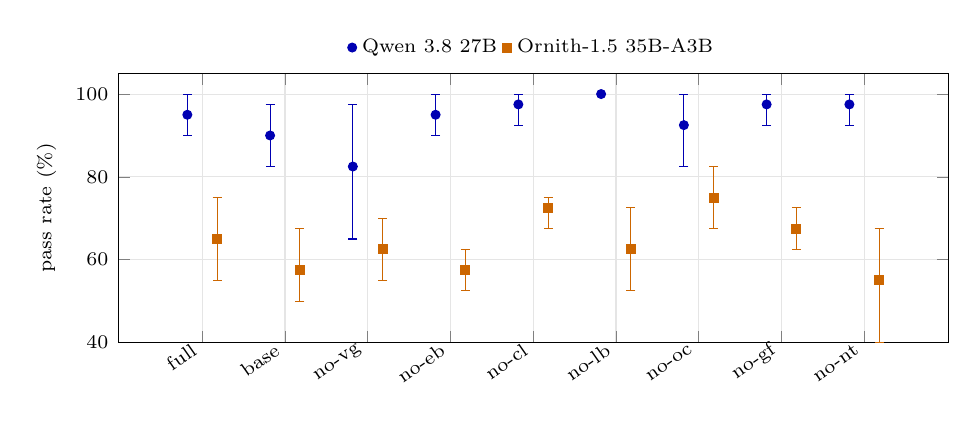
\begin{tikzpicture}
\begin{axis}[
  width=\linewidth, height=5.0cm,
  ymin=40, ymax=105, ylabel={pass rate (\%)},
  xtick={0,1,2,3,4,5,6,7,8}, xticklabels={full,base,no-vg,no-eb,no-cl,no-lb,no-oc,no-gf,no-nt},
  x tick label style={font=\scriptsize,rotate=35,anchor=east},
  y tick label style={font=\scriptsize},
  ylabel style={font=\scriptsize},
  legend style={font=\scriptsize,at={(0.5,1.02)},anchor=south,legend columns=2,draw=none},
  grid=major, grid style={gray!20},
  error bars/y dir=both, error bars/y explicit,
]
\addplot[only marks,mark=*,mark size=1.6pt,color=blue!70!black] coordinates {
(-0.18,95.0) +- (0,5.0) -= (0,5.0)
(0.82,90.0) +- (0,7.5) -= (0,7.5)
(1.82,82.5) +- (0,15.0) -= (0,17.5)
(2.82,95.0) +- (0,5.0) -= (0,5.0)
(3.82,97.5) +- (0,2.5) -= (0,5.0)
(4.82,100.0) +- (0,0.0) -= (0,0.0)
(5.82,92.5) +- (0,7.5) -= (0,10.0)
(6.82,97.5) +- (0,2.5) -= (0,5.0)
(7.82,97.5) +- (0,2.5) -= (0,5.0)
};
\addlegendentry{Qwen 3.8 27B}
\addplot[only marks,mark=square*,mark size=1.6pt,color=orange!80!black] coordinates {
(0.18,65.0) +- (0,10.0) -= (0,10.0)
(1.18,57.5) +- (0,10.0) -= (0,7.5)
(2.18,62.5) +- (0,7.5) -= (0,7.5)
(3.18,57.5) +- (0,5.0) -= (0,5.0)
(4.18,72.5) +- (0,2.5) -= (0,5.0)
(5.18,62.5) +- (0,10.0) -= (0,10.0)
(6.18,75.0) +- (0,7.5) -= (0,7.5)
(7.18,67.5) +- (0,5.0) -= (0,5.0)
(8.18,55.0) +- (0,12.5) -= (0,15.0)
};
\addlegendentry{Ornith-1.5 35B-A3B}
\end{axis}
\end{tikzpicture}

\caption{Every cell of the one-flag ladder with bootstrap 95\% intervals, generated directly
from the statistics file. Neither model peaks at \texttt{full}: Qwen is highest at
\texttt{no-loopbreak} and Ornith at \texttt{no-outcap}. Intervals overlap almost everywhere ---
that overlap is the result, not a presentation problem.}
\label{fig:ladder}
\end{figure}

\paragraph{The bundle is not the optimum, and one component hurts.}
Table~\ref{tab:ladder} is the result we did not expect. \emph{Neither model's best
configuration is \texttt{full}}: Qwen peaks at \texttt{no-loopbreak} (100\%, every seed on every
task) and Ornith at \texttt{no-outcap} (75.0\%). Removing the output cap raises the weaker
model with $\Delta = -10.0$, CI $[-17.5, -2.5]$ --- the only interval in the ladder excluding
zero, and it says a component we shipped was costing us. The mechanism is legible: Ornith is
the model living near its context ceiling, and truncating a tool result does not reduce its
prompt growth so much as remove the evidence it needed, while the truncation notice itself
costs tokens. A practitioner shipping the full bundle because each component has a plausible
story is shipping two components that cost their model episodes.

\begin{figure}[t]
\centering
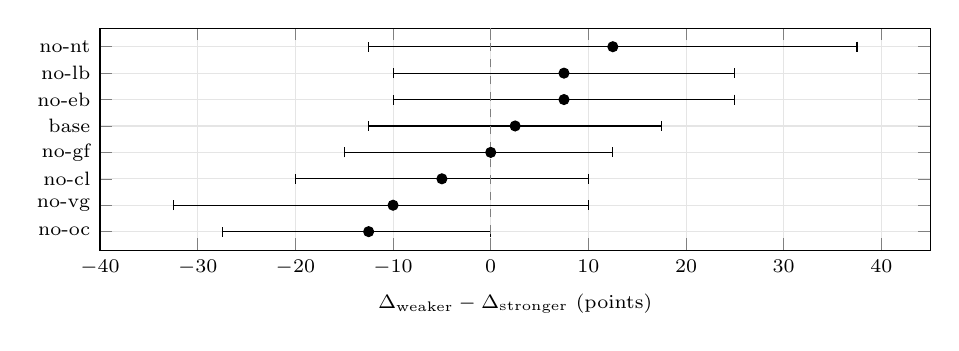
\begin{tikzpicture}
\begin{axis}[
  width=\linewidth, height=4.4cm,
  xmin=-40, xmax=45, xlabel={$\Delta_{\mathrm{weaker}}-\Delta_{\mathrm{stronger}}$ (points)},
  ytick={0,1,2,3,4,5,6,7}, yticklabels={no-oc,no-vg,no-cl,no-gf,base,no-eb,no-lb,no-nt},
  y tick label style={font=\scriptsize}, x tick label style={font=\scriptsize},
  xlabel style={font=\scriptsize},
  ymin=-0.7, ymax=7.7,
  grid=major, grid style={gray!20},
  error bars/x dir=both, error bars/x explicit,
]
\addplot[only marks,mark=*,mark size=1.8pt,color=black] coordinates {
(-12.5,0) +- (12.5,0) -= (15.0,0)
(-10.0,1) +- (20.0,0) -= (22.5,0)
(-5.0,2) +- (15.0,0) -= (15.0,0)
(0.0,3) +- (12.5,0) -= (15.0,0)
(2.5,4) +- (15.0,0) -= (15.0,0)
(7.5,5) +- (17.5,0) -= (17.5,0)
(7.5,6) +- (17.5,0) -= (17.5,0)
(12.5,7) +- (25.0,0) -= (25.0,0)
};
\draw[dashed,gray] (axis cs:0,-0.7) -- (axis cs:0,7.7);
\end{axis}
\end{tikzpicture}

\caption{The interaction test, sorted by point estimate. Every interval crosses zero and the
estimates disagree in sign. This is what an underpowered test looks like; it is not evidence
that the interaction is absent.}
\label{fig:interaction}
\end{figure}

\paragraph{The interaction is undetectable.}
The hypothesis motivating harness engineering is that structure matters more for weaker models.
Assigning arms empirically (Ornith 65.0\% weaker, Qwen 95.0\% stronger), all eight
$\Delta_{\text{weaker}} - \Delta_{\text{stronger}}$ intervals include zero, and the point
estimates do not agree in sign: four positive, three negative, one exactly zero. We report this
as underpowered rather than absent (Figure~\ref{fig:interaction}).

\paragraph{How underpowered, exactly.}
"Underpowered" is only useful with a number attached. Resampling each contrast's observed
per-seed spread and asking how often a bootstrap interval would exclude zero gives the seed
counts a follow-up would need:

\begin{center}\small
\begin{tabular}{lrrrr}
\toprule
Contrast & $n{=}5$ & $n{=}10$ & $n{=}20$ & $n{=}40$ \\
\midrule
Qwen full vs.\ baseline             & 33\% & 70\% & 98\% & 100\% \\
Ornith full vs.\ baseline           & 19\% & 31\% & 60\% & 89\% \\
Ornith \texttt{no-outcap}           & 68\% & 96\% & 100\% & 100\% \\
Interaction, \texttt{no-outcap}     & 38\% & --- & 86\% & --- \\
Interaction, \texttt{no-verifygate} & 33\% & --- & 99\% & --- \\
\bottomrule
\end{tabular}
\end{center}

\noindent Twenty seeds --- four times this grid, roughly 2{,}900 episodes --- would resolve most
of these, and the one result already significant (\texttt{no-outcap}) was detectable at the $n$
we ran. This is a sample-size problem with a known price, not an unfalsifiable one. What extra
seeds would \emph{not} fix is construct validity: eight Python tasks written by the harness
author, a one-flag-at-a-time design blind to interactions between flags, and a weaker arm whose
failures are dominated by context exhaustion. Those need different tasks and a different design,
not more compute.

\paragraph{Cost is not wall-clock.}
We make no timing claim: some cells shared the GPU and later ones did not. What the transcripts
support is step count --- on one task the full harness finished in 14--17 steps against a
baseline of 35--40, the baseline's median being the turn ceiling itself. A 43.8-hour telemetry
log (78{,}027 samples) shows the serial batch-1 loop drawing a median 302\,W against the
GH200's 900\,W cap while \texttt{utilization.gpu} reads 89\%, with the SM clock pinned at
maximum in 78{,}025 of 78{,}027 samples. Utilization near 90\% here means a decode that cannot
fill the device, not saturation --- anyone budgeting agent-grid GPU-hours from a utilization
percentage will misread what the device is doing.

\subsection{A gate catches what a prompt does not}
\label{sec:gate}

The grid ablates a bundle; one task isolates the gate against a legible failure. Its visible
test checks a printed total; the hidden tests also check that a loader returns values already
converted from cents, which is that module's documented contract. Without the gate the model
often satisfies the visible test by breaking the contract --- writing the loader to return raw
cent arrays --- then calls \texttt{finish} satisfied. Across matched configurations differing
only in this flag, the model passes 9/9 with the gate and 5/9 without (Fisher exact
$p = 0.082$); pooling adjacent single-episode tags gives 10/10 versus 7/13 ($p = 0.019$). We
report both and lead with the conservative count, which does not reach $\alpha = 0.05$.

The mechanism is cleaner than the counts. Of every no-gate failure logged on this task,
\emph{all} stopped with \texttt{stop\_reason = finished}: not one was a crash, a timeout, or an
exhausted context. Every failure was the model asserting completion on work that did not pass.
Notably the prompt-side checklist was \textbf{on in both arms} --- it asks directly whether any
test was weakened and whether the fix addresses the cause --- and did not prevent the false
finish. Only the external check did. That is a data point against prompt-level mitigation of
shortcut-taking \citep{everymodel} and in favour of a structural gate.

\section{What honest measurement costs}
\label{sec:cost}

Two failure modes bit us. Neither is visible in a pass rate, and both would have produced a
more impressive paper.

\paragraph{A protocol change masquerading as an effect.}
Our first 160 episodes used a 40-turn ceiling; we then removed it, kept already-passing
episodes, and re-ran only the ceiling failures. Under that mix the same contrast reads
$+22.5$ points with CI $[+10.0, +37.5]$ --- \emph{excluding zero}, four times the frozen effect,
and far more publishable. It is an artifact: the baseline still contained 40-step leftovers.
The tell is in the archive, where the baseline's maximum step count is exactly 40, the old
ceiling, while the frozen re-run reaches 48. A 17.5-point swing in the headline came entirely
from which turn ceiling the baseline had been run under.

\paragraph{Censoring that correlates with difficulty.}
We tried to add a third, API-served rung. Our first sweep produced 315 episodes with
\emph{zero} successful finishes; the cause was our own client, which sent tool results with no
preceding tool-call record, so the model lost its action history every turn. After fixing that,
episodes behaved normally (14--25 tool calls, clean finishes) but 32.5\% of requests were
refused by the endpoint under load. Those refusals were not random with respect to the outcome:
one task was refused on every attempt, and both stronger models pass it 5/5. We excluded the
arm. The reason is not the error rate --- we keep serving errors in the denominator elsewhere,
on the assumption that they are noise. Here they are not: they systematically censor the tasks
requiring the most generated code. Any ablation $\Delta$ would be confounded, because flags that
change how much the model writes in one call would move the refusal rate and read as a harness
effect. \emph{An error rate is reportable; an error rate correlated with difficulty is not.}

\section{Limitations and conclusion}

Five repeats per cell: fifteen of sixteen paired intervals include zero, and a percentile
bootstrap on five points describes observed spread rather than carrying reliable coverage. Two
models, both local and quantized, spanning 65--95\% on one suite. The weaker arm ends 45\% of
its full-harness episodes in context exhaustion or serving errors, mixing capability with
serving fragility. Eight Python tasks written by the same author as the harness, a bias toward
failures this harness was built to catch. The design is one-flag-at-a-time, so components that
only pay together, or that cancel, are invisible.

We described a coding harness small enough to run around a local 27B model and factored enough
that its components can be measured rather than assumed. Turning the full bundle on raised the
stronger model by 5.0 points with an interval including zero; the bundle is not optimal for
either model; the one component whose interval excludes zero was \emph{hurting} the weaker
model; and the capability-by-harness interaction is undetectable at this $n$. The contribution
we are most confident in is not an effect size. It is that a harness written as a bag of flags,
with an external grader and an honest stop-reason field, converts questions usually settled by
leaderboard position into questions with intervals --- including the uncomfortable answer that
most of them do not have one yet.

\paragraph{Reproducibility.} Harness, tasks, runner, and statistics are dependency-free Python.
Every table regenerates from one command, and figures render from the same statistics file, so
a figure cannot disagree with a table. Archived runs carry provenance notes recording what they
are and whether they may be used.

\small
\bibliographystyle{plainnat}
\begin{thebibliography}{99}\itemsep1pt
\bibitem[Lee et al.(2026)]{metaharness} Y.~Lee, R.~Nair, Q.~Zhang, K.~Lee, O.~Khattab, and C.~Finn. Meta-Harness: End-to-end optimization of model harnesses. \emph{arXiv:2603.28052}, 2026.
\bibitem[Merrill et al.(2026)]{terminalbench} M.~A. Merrill et al. Terminal-Bench: Benchmarking agents on hard, realistic tasks in command line interfaces. \emph{arXiv:2601.11868}, 2026.
\bibitem[KRAFTON AI(2026)]{terminuskira} KRAFTON AI and Ludo Robotics. Terminus-KIRA: Boosting frontier model performance on Terminal-Bench with a minimal harness. 2026. As cited by \citet{metaharness}.
\bibitem[Yang et al.(2024)]{sweagent} J.~Yang, C.~E. Jimenez, A.~Wettig, K.~Lieret, S.~Yao, K.~Narasimhan, and O.~Press. SWE-agent: Agent-computer interfaces enable automated software engineering. In \emph{NeurIPS}, 2024.
\bibitem[Xia et al.(2024)]{agentless} C.~S. Xia, Y.~Deng, S.~Dunn, and L.~Zhang. Agentless: Demystifying LLM-based software engineering agents. \emph{arXiv:2407.01489}, 2024.
\bibitem[Zhang et al.(2024)]{autocoderover} Y.~Zhang, H.~Ruan, Z.~Fan, and A.~Roychoudhury. AutoCodeRover: Autonomous program improvement. In \emph{ISSTA}, 2024.
\bibitem[Aleithan et al.(2024)]{swebenchplus} R.~Aleithan, H.~Xue, M.~M. Mohajer, E.~Nnorom, G.~Uddin, and S.~Wang. SWE-Bench+: Enhanced coding benchmark for LLMs. \emph{arXiv:2410.06992}, 2024.
\bibitem[Lodkaew et al.(2026)]{deceive} T.~Lodkaew, J.~Ackermann, S.~Nishimori, N.~Charoenphakdee, M.~Sugiyama, and T.~Ishida. Do coding agents deceive us? Detecting and preventing cheating via capped evaluation with randomized tests. \emph{arXiv:2606.07379}, 2026.
\bibitem[Kouremetis et al.(2026)]{everymodel} M.~Kouremetis, A.~Dawson, R.~S.~R. Dheekonda, and B.~Greunke. Every model cheats: Prompt-level mitigation of cheating on offensive cyber tasks. \emph{arXiv:2607.21763}, 2026.
\bibitem[Chen et al.(2023)]{selfdebug} X.~Chen, M.~Lin, N.~Sch\"arli, and D.~Zhou. Teaching large language models to self-debug. \emph{arXiv:2304.05128}, 2023.
\bibitem[Li et al.(2024)]{ldb} Z.~Li, Z.~Wang, and J.~Shang. Debug like a human: A large language model debugger via verifying runtime execution step by step. In \emph{Findings of ACL}, 2024.
\bibitem[Liu et al.(2024)]{lostmiddle} N.~F. Liu, K.~Lin, J.~Hewitt, A.~Paranjape, M.~Bevilacqua, F.~Petroni, and P.~Liang. Lost in the middle: How language models use long contexts. \emph{TACL}, 12, 2024.
\bibitem[Nicholson(2026)]{drift} C.~Nicholson. Quantifying non-deterministic drift in large language models. \emph{arXiv:2601.19934}, 2026.
\bibitem[DiCiccio and Efron(1996)]{bootstrap} T.~J. DiCiccio and B.~Efron. Bootstrap confidence intervals. \emph{Statistical Science}, 11(3):189--228, 1996.
\end{thebibliography}

\end{document}
